%% EduGuard — Elsevier elsarticle-style manuscript (Overleaf-ready)
%% Same verified numbers as the IEEE manuscript. Edit author metadata before submission.
\documentclass[review,12pt]{elsarticle}
\usepackage{amssymb,amsmath}
\usepackage{graphicx}
\usepackage{booktabs}
\usepackage{hyperref}
\usepackage{lineno}
\modulolinenumbers[5]

\journal{Computers and Education / Expert Systems with Applications (select at submission)}

\graphicspath{{figures/}{../figures/}{../../artifacts/evaluation/paper/}}

\begin{document}

\begin{frontmatter}

\title{A Lightweight Multi-Modal Tiny LLM Framework for Privacy-Preserving Academic Assistance in University Environments}

\author[aff1]{Author One}
\author[aff1]{Author Two}

\affiliation[aff1]{organization={University Affiliation},
            addressline={Address},
            city={City},
            country={Country}}

\begin{abstract}
EduGuard is an offline-oriented academic assistance system that keeps Bloom-level classification, multitask generation, retrieval, and protected-content screening as separate modules.
A Qwen2.5-0.5B sequence classifier predicts Bloom taxonomy levels and validates rewritten questions.
A Qwen2.5-1.5B causal model trained under the locked multitask \emph{v3} protocol performs target-level rewriting, question answering, and summarization.
Federated FedAvg/FedProx experiments train the classifier without centralizing raw client training text in the simulation.
On Figshare Bloom test data ($N{=}350$), the selected FedProx IID checkpoint (validation-best round 20) reaches accuracy $0.8057$ and macro-F1 $0.7982$, compared with centralized LoRA accuracy $0.8314$ in the same evaluation artifact family.
On the frozen multitask test set ($N{=}8321$), v3 Bloom target agreement is $0.8880$ when scored by the merged 0.5B classifier and $0.9518$ when the same generations are rescored by the federated classifier (\texttt{classifier\_is\_not\_ground\_truth=true}).
QA token F1 is $0.7854$; summarization ROUGE-L is $0.1496$.
The generator deploys as Q4\_K\_M GGUF ($986{,}048{,}032$ bytes; $28.89$ tokens/s in the recorded micro-benchmark).
PrivacyGuard blocks all $104$ taxonomy attacks in the current artifact but admits none of $15$ benign student prompts.
We do not claim formal differential privacy.
\end{abstract}

\begin{keyword}
Bloom's taxonomy \sep federated learning \sep LoRA \sep educational question rewriting \sep local LLM inference \sep retrieval-augmented generation \sep privacy-aware education systems
\end{keyword}

\end{frontmatter}

\linenumbers

\section{Introduction}
Assessment design frequently relies on Bloom's cognitive levels~\cite{bloom1956taxonomy,anderson2001revision}.
Teachers may wish to rewrite a stem toward a higher or lower level, classify existing items, and answer student questions over approved materials---while keeping protected exam banks off shared servers.
EduGuard addresses this setting with three deliberate separations: (1)~a small sequence classifier for Bloom labels, (2)~a larger causal multitask generator, and (3)~role-aware retrieval with empirical output/query screening.

The manuscript reports only results that survive provenance checks in the EduGuard repository.
Earlier multitask experiments on an older synthetic rewrite corpus are treated as historical development runs and are excluded from primary tables.
Formal differential privacy is discussed only as an incomplete line of work: a DP federated run exists with near-chance accuracy and is not used as a positive claim~\cite{abadi2016dpsgd}.

\section{Related work}

\subsection{Small and local language models}
Task-specific small language models can match larger cloud models on narrow educational tasks while remaining locally hosted~\cite{slm2026teammates,saur2026grading,tinyllm2024,localai2026}.
In-domain gains do not automatically transfer, and LLM-as-judge scores can disagree with expert ratings~\cite{slm2026teammates,saur2026grading}.
Local deployment is a governance property~\cite{bogicevic2026rag,localai2026}, not a privacy proof.
EduGuard uses Qwen2.5-0.5B for classification and Qwen2.5-1.5B, later Q4\_K\_M GGUF, for generation~\cite{qwen2024technical}.

\subsection{Retrieval-augmented generation}
RAG grounds answers in retrieved text~\cite{lewis2020rag}.
Educational systems have used RAG for campus deployment~\cite{bogicevic2026rag} and for Bloom-structured assessment~\cite{ragcognitive2025}.
Neither shows that retrieval alone stops leakage of confidential exam wording.
EduGuard keeps separate public and protected FAISS indexes~\cite{johnson2019faiss} with BGE-family embeddings~\cite{xiao2024bge}.
Role gating is independent of the retriever's privacy-weighted score.
A complete Recall@k/MRR benchmark is not available, so retrieval is reported as an implemented path, not as a measured retrieval result.
QA uses SQuAD-style exact match and token F1~\cite{rajpurkar2016squad}; summarization uses ROUGE~\cite{lin2004rouge}.

\subsection{Bloom classification and question rewriting}
Objective and question classification spans classical features, transformers, and prompted LLMs~\cite{li2022objectives,mohammed2020tfidf,waheed2021bloomnet,bloomanalysis2025,crossbloom2026,abduljabbar2015bloom}.
Cross-dataset generalization is a recurring weakness~\cite{waheed2021bloomnet,crossbloom2026}.
Much of that work uses the original Bloom categories.
This study uses the revised six levels~\cite{bloom1956taxonomy,anderson2001revision} and reports quadratic weighted kappa~\cite{cohen1968weighted}.
Bloom-targeted generation is established~\cite{teachers2024quizzes,bea2024questions,qgen2024strategies,gpt4answers2024}, but those studies usually write new items from a topic.
They do not evaluate classify-then-rewrite-then-reclassify on an existing question.
EduGuard's reclassification step is automatic and is not a human rating.

\subsection{LoRA, federated learning, and differential privacy}
Both models use LoRA~\cite{hu2022lora}.
QLoRA~\cite{dettmers2023qlora,teachinglora,spamqlora2026} and other PEFT methods~\cite{sktuning2024} are not the training method used here.
The classifier uses rank $32$ ($\alpha{=}64$); the v3 generator uses rank $16$ ($\alpha{=}32$).
Quantization is post-training and applies only to the generator.
FedAvg~\cite{mcmahan2017fedavg,konecny2016comm} and FedProx~\cite{li2020fedprox} train the classifier.
Client-adaptive federated LoRA methods~\cite{flexlora2024,lorafair2024} are not implemented.
On the locked IID 20-round test, FedProx accuracy is $0.8057$ and FedAvg is $0.8000$.
On the five-round Dirichlet $\alpha{=}0.5$ split, FedProx ($0.4571$) does not exceed FedAvg ($0.5029$) at $\mu{=}0.01$.
That is a statistical-heterogeneity observation, not a replication of FedProx gains under systems heterogeneity~\cite{li2020fedprox}.
Federated optimization is not differential privacy~\cite{alrubaie2018privacy,kairouz2021advances,abadi2016dpsgd}.
The DP-SGD FedProx run (accuracy $0.1286$) was not adopted.

\subsection{Gap addressed}
The papers above treat local SLMs, Bloom classification, question generation, RAG, LoRA, and federated learning separately.
This work integrates role-separated retrieval, an empirical content screen, a federated 0.5B revised-taxonomy classifier, and a separate 1.5B rewrite generator.
It does not claim a new learning algorithm or a formal privacy definition.

\section{System architecture}
Figure~\ref{fig:arch} shows the implemented configuration.
Student sessions resolve to the public corpus.
Teacher sessions may use authorized protected indexes in the role model.
Target-level rewriting uses question + target Bloom level as generator inputs; source Bloom is analysis metadata only.
The 0.5B classifier validates predicted cognitive level after generation.
Only the 1.5B causal model is quantized to GGUF; the classifier remains a Hugging Face sequence-classification component.

\begin{figure*}[t]
\centering
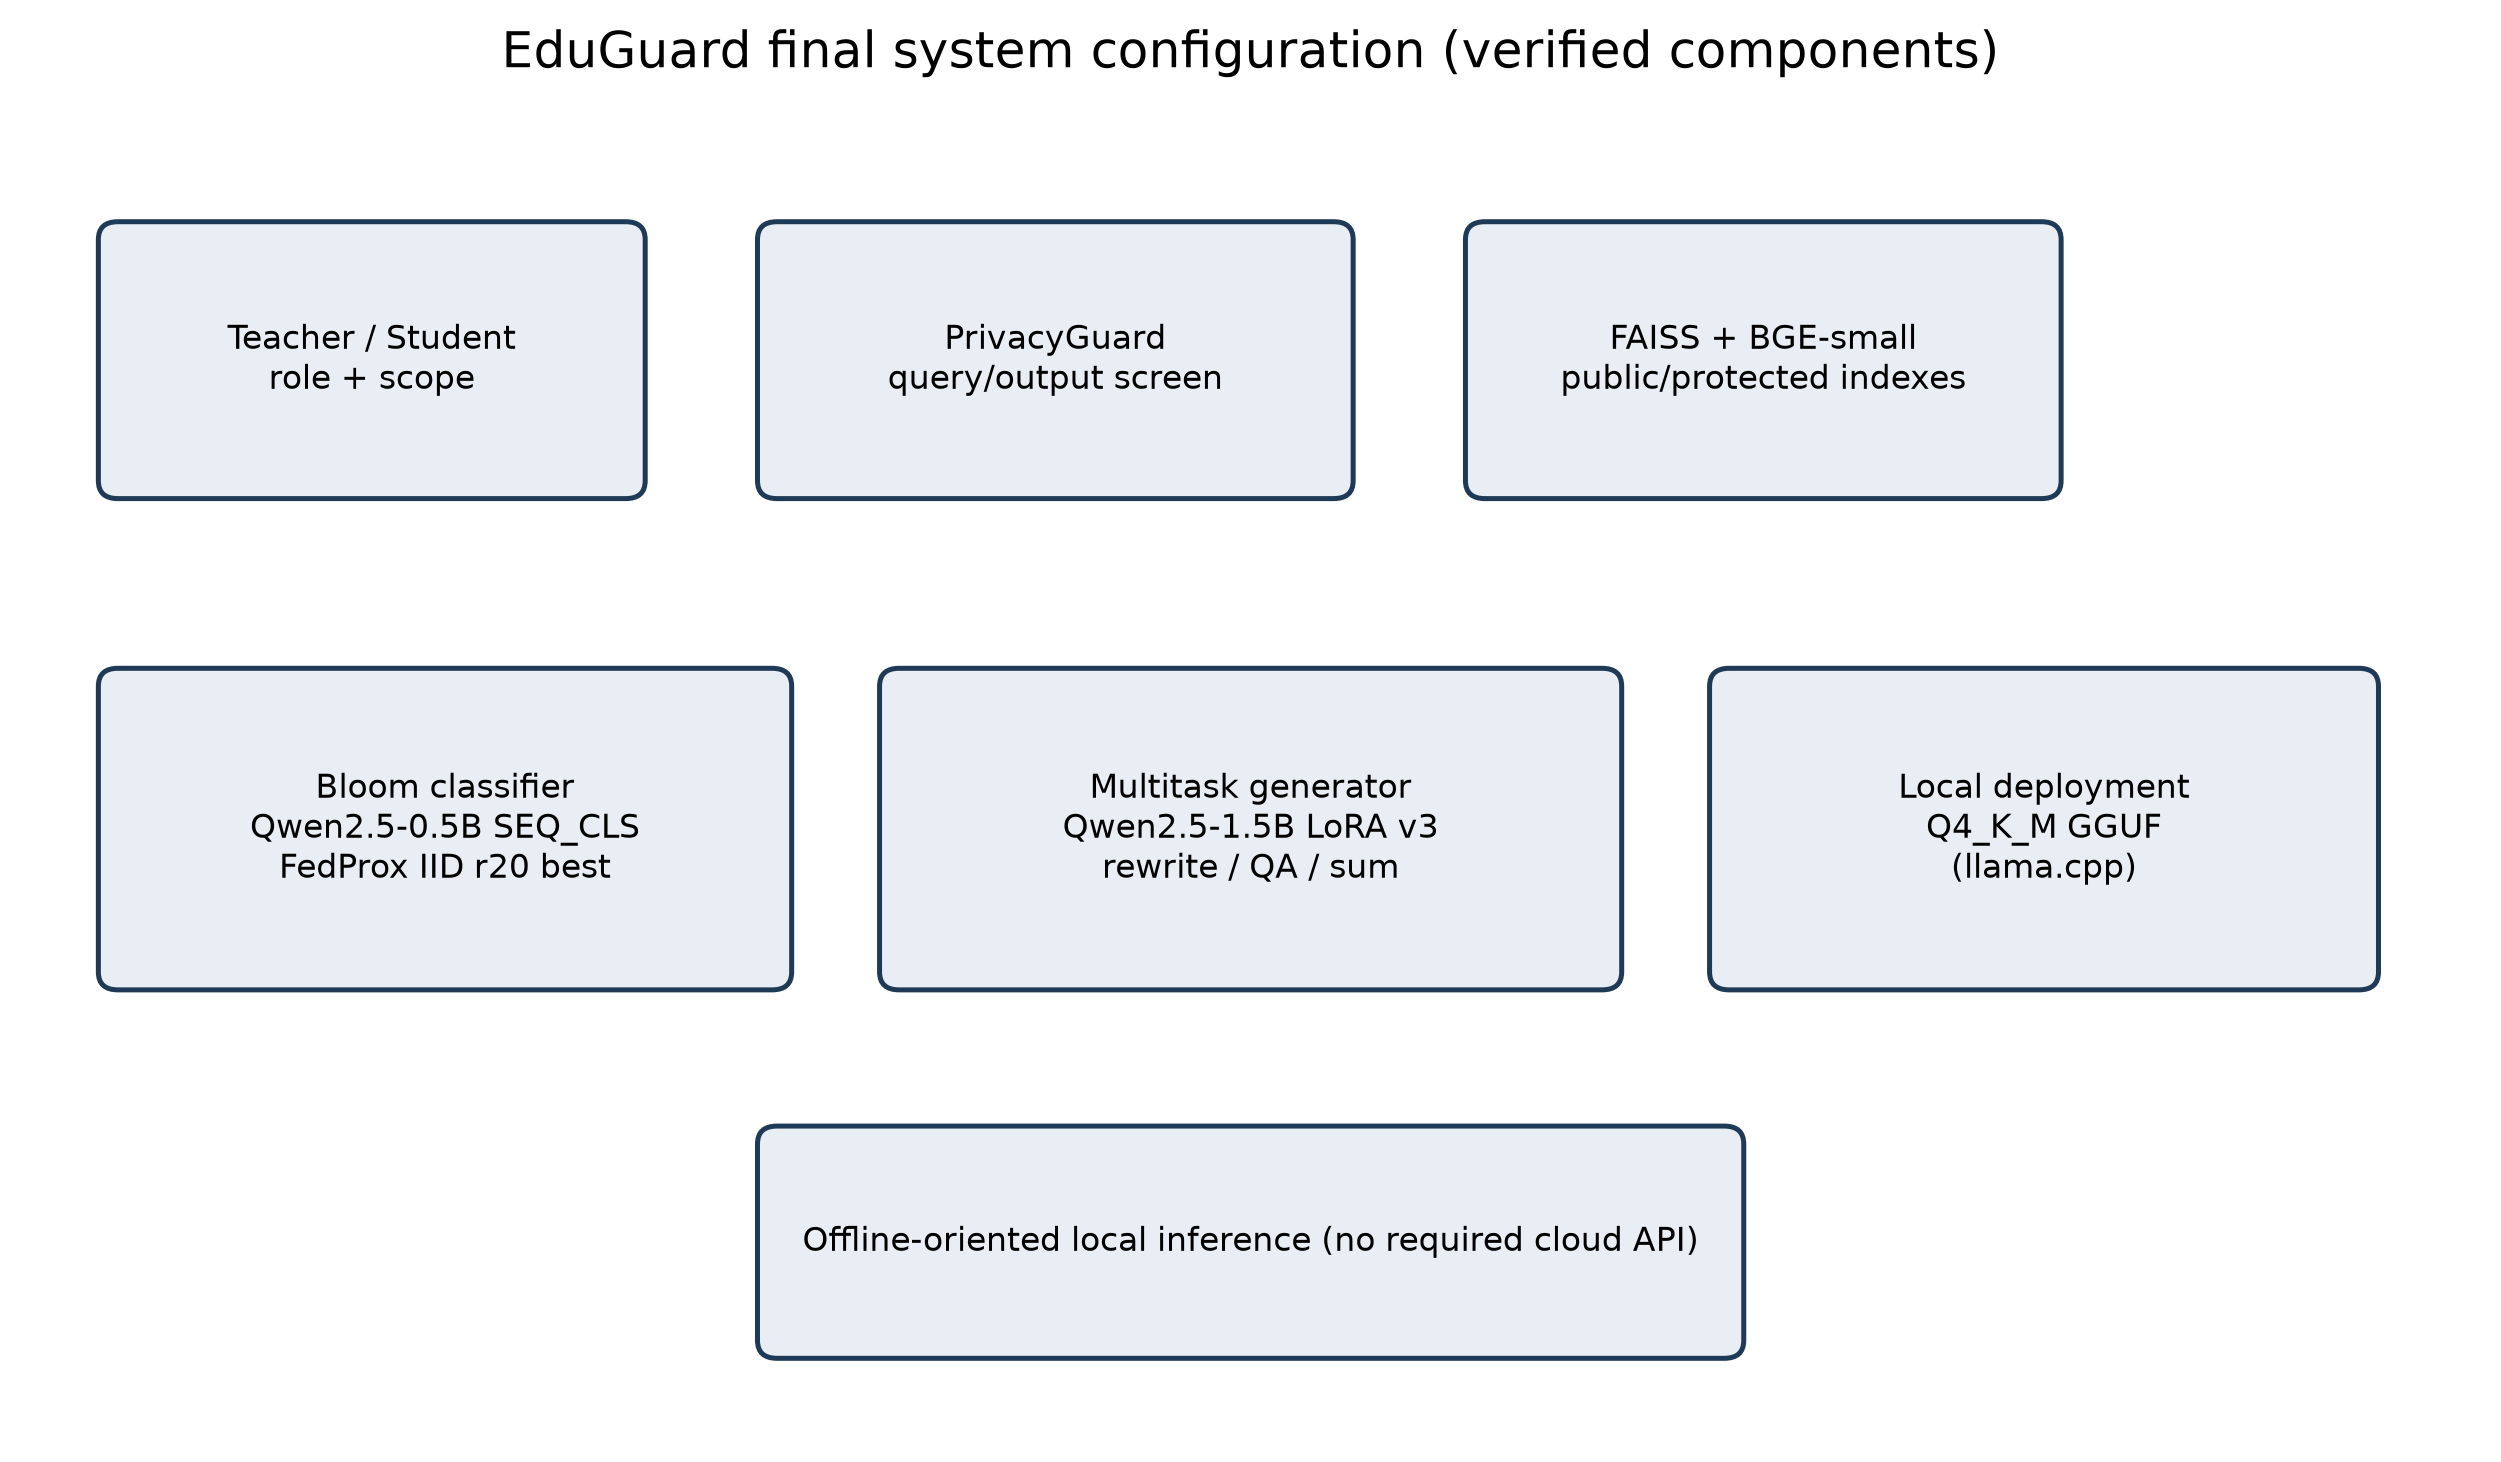
\includegraphics[width=0.92\textwidth]{fig01_system_architecture.png}
\caption{Verified EduGuard modules: classifier, multitask generator, RAG indexes, roles, and PrivacyGuard.}
\label{fig:arch}
\end{figure*}

\section{Methods}

\subsection{Bloom classifier}
Qwen2.5-0.5B-Instruct is fine-tuned for six-way sequence classification with LoRA ($r{=}32$, $\alpha{=}64$, dropout $0.1$) and a saved score head.
The training split is imbalanced (Understand $640$, Remember $225$, Evaluate $199$, Apply $199$, Analyze $192$, Create $176$ of $1631$).
Sequence length is capped at $256$ tokens.
Dynamic INT8 quantization is rejected in repository code due to accuracy collapse; FP16 merged export is documented instead.
A recorded McNemar test against a 1.5B reference yields $p{=}0.711071$ ($n_{\mathrm{discordant}}{=}29$), but full 1.5B metrics JSON files are missing, so 1.5B accuracy is not tabulated.
The classifier labels questions and rewrites; it does not generate them.

\subsection{Federated training}
Eight simulated clients; FedAvg and FedProx ($\mu{=}0.01$); IID and Dirichlet non-IID partitions where executed; local epochs $3$; seed $42$.
Model selection maximizes validation accuracy.
Test metrics are computed on Figshare held-out items ($N{=}350$).

\subsection{Multitask v3 generator}
Qwen2.5-1.5B-Instruct with multitask LoRA (rank $16$) on Mix-A data.
Bloom rewrite stems use synthetic policy v3 transformations.
Training/eval decoding for reported metrics uses greedy generation with \texttt{max\_new\_tokens}${}={}128$.
Pre-v3 result directories (\texttt{qwen05b\_lora}, \texttt{qwen15b\_lora}, \texttt{qwen15b\_lora\_sumfix}) are excluded from main claims following the repository diagnosis of format/answer-output failures and synth\_v2 template weaknesses.
The teacher workflow classifies an input, rewrites it to a specified target level, and re-scores the output.
That re-score is automatic.
Human Bloom-alignment ratings were not collected.

\subsection{Privacy and roles}
Student sessions use the public index only.
Teacher sessions may use an authorized protected scope.
PrivacyGuard combines regex patterns, n-gram and span overlap, semantic-concept checks, and an auxiliary risk score.
Reported rates come from the locked $104$-attack taxonomy artifact.
Local GGUF inference is an offline-oriented deployment choice for the generator only; it is not a privacy mechanism.
These controls are empirical, not cryptographic, and not differential privacy.

\section{Experimental setup}
Figshare Bloom: $1631$/$349$/$350$ train/val/test.
Multitask frozen test: $8321$ examples (Bloom $1536$, QA $5285$, summarization $1500$), SHA256 \texttt{1eb88cd5900fcb9154cbf70e6a62d49636c9ad882aa5d8e303285524c74cc391}.
v3 train total $6466$.
Leakage overlaps reported as zero in evaluation metadata.

\section{Results}

\subsection{Classification and federated learning}
Table~\ref{tab:bloom} lists locked metrics.
FedProx IID r20 (best round 20) is the selected classifier: accuracy $0.8057$, macro-F1 $0.7982$, QWK $0.8493$, within-one $0.9086$, severe error $0.0429$, ECE $0.0537$ (live evaluation; stored training-run ECE $0.0565$).
Centralized LoRA accuracy is $0.8314$ (gap $-2.57$ percentage points).
FedAvg best-test accuracy is $0.8000$ (best round 15).
Non-IID five-round accuracy falls to $0.5029$ (FedAvg, $\alpha{=}0.5$) and $0.4571$ (FedProx, $\alpha{=}0.5$).

\begin{table}[t]
\centering
\caption{Bloom classifier results on Figshare test ($N{=}350$).}
\label{tab:bloom}
\begin{tabular}{lcccccc}
\toprule
Model & Acc & Macro-F1 & QWK & Within-1 & Severe & ECE \\
\midrule
TF-IDF+SVM & 0.7514 & 0.7253 & 0.7471 & 0.8829 & 0.0657 & --- \\
Central 0.5B LoRA & 0.8314 & 0.8252 & 0.8794 & 0.9200 & 0.0371 & 0.0542 \\
FedAvg r20 best & 0.8000 & 0.7920 & 0.8412 & 0.8943 & 0.0486 & 0.0395 \\
FedProx r20 best & 0.8057 & 0.7982 & 0.8493 & 0.9086 & 0.0429 & 0.0537 \\
\bottomrule
\end{tabular}
\end{table}

\begin{figure}[t]
\centering
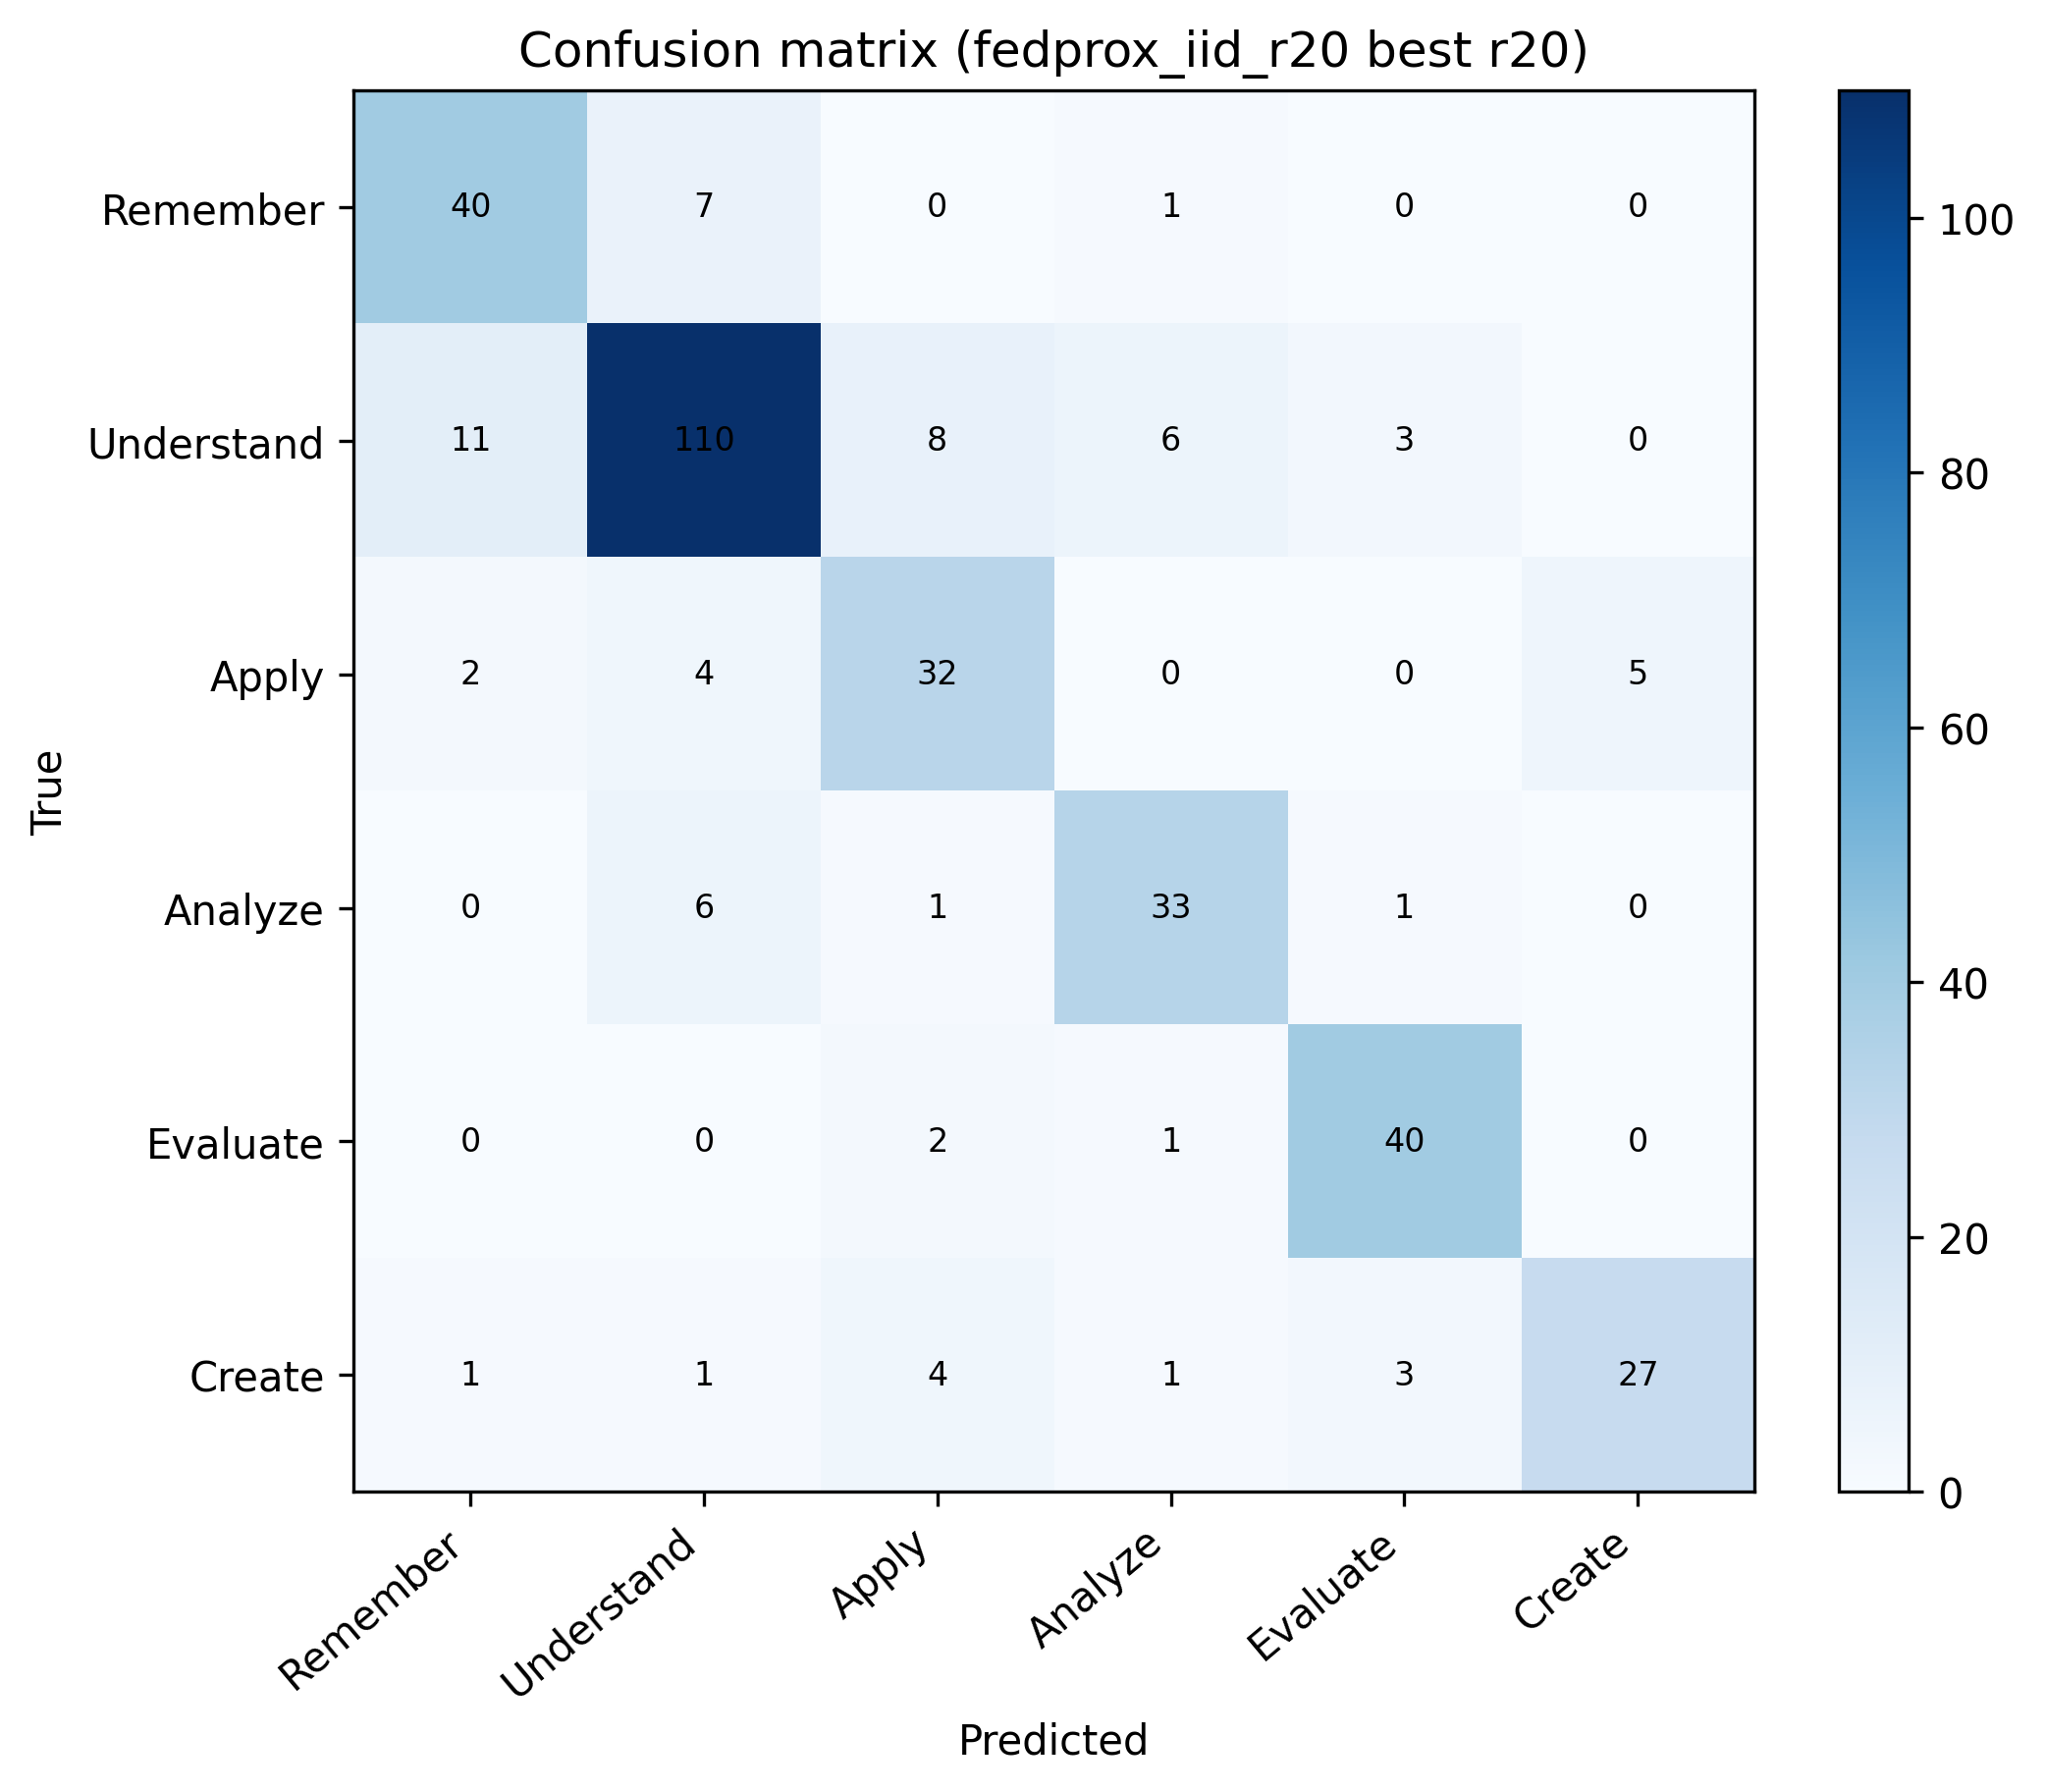
\includegraphics[width=\columnwidth]{fig02_bloom_confusion_matrix.png}
\caption{FedProx r20 confusion matrix ($N{=}350$).}
\label{fig:cm}
\end{figure}

\begin{figure}[t]
\centering
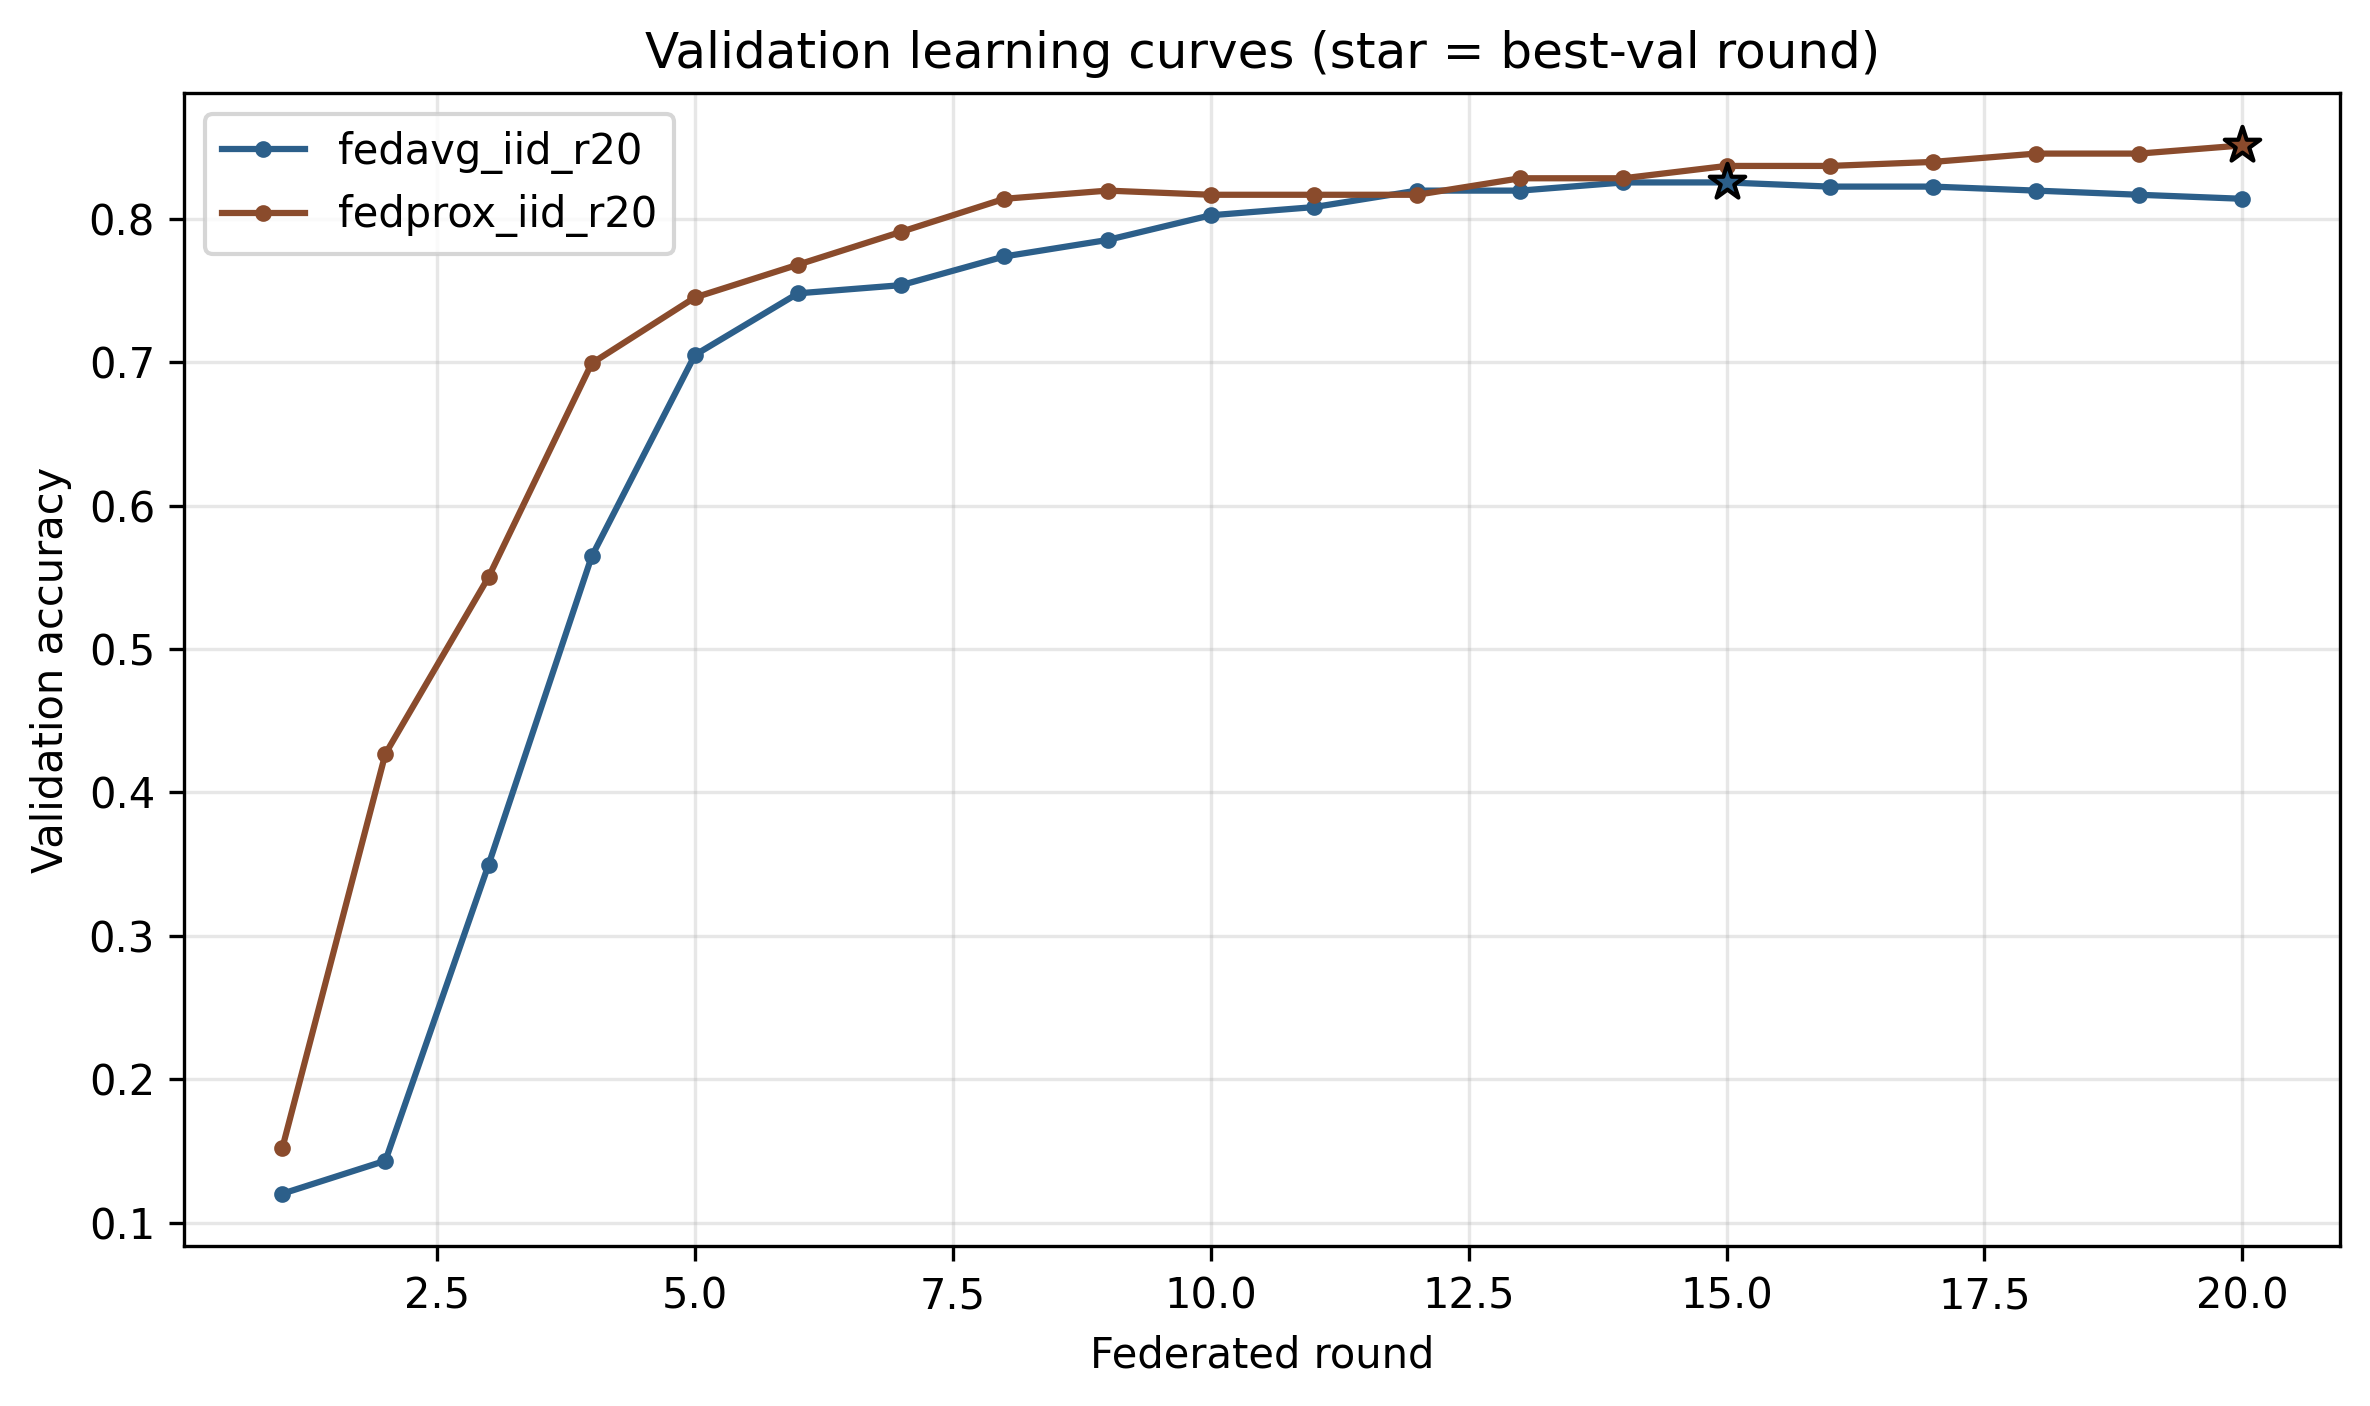
\includegraphics[width=\columnwidth]{fig03_fedavg_fedprox_learning_curves.png}
\caption{FedAvg vs FedProx learning curves (20-round IID).}
\label{fig:curves}
\end{figure}

\subsection{Multitask generation}
Table~\ref{tab:mt} summarizes v3.
Summarization is weaker than rewrite and QA under the retained limits.
A historical longer-context ablation improved ROUGE/QA but reduced fully-validated and cognitive rates; primary v3 ($512$/$128$) was kept for rewrite validation priority.

\begin{table}[t]
\centering
\caption{Multitask v3 frozen-test metrics. Classifier agreement is automatic, not human ground truth.}
\label{tab:mt}
\begin{tabular}{llr}
\toprule
Task & Metric & Value \\
\midrule
Bloom rewrite ($N{=}1536$), merged 0.5B scorer & Target accuracy & 0.8880 \\
 & Macro-F1 & 0.8768 \\
 & Fully validated & 0.7070 \\
Bloom rewrite, FedProx scorer (same text) & Target accuracy & 0.9518 \\
 & Macro-F1 & 0.9443 \\
 & Fully validated & 0.7624 \\
QA ($N{=}5285$) & Exact match & 0.5784 \\
 & Token F1 & 0.7854 \\
Summarization ($N{=}1500$) & ROUGE-1 & 0.2491 \\
 & ROUGE-2 & 0.0573 \\
 & ROUGE-L & 0.1496 \\
\bottomrule
\end{tabular}
\end{table}

\begin{figure}[t]
\centering
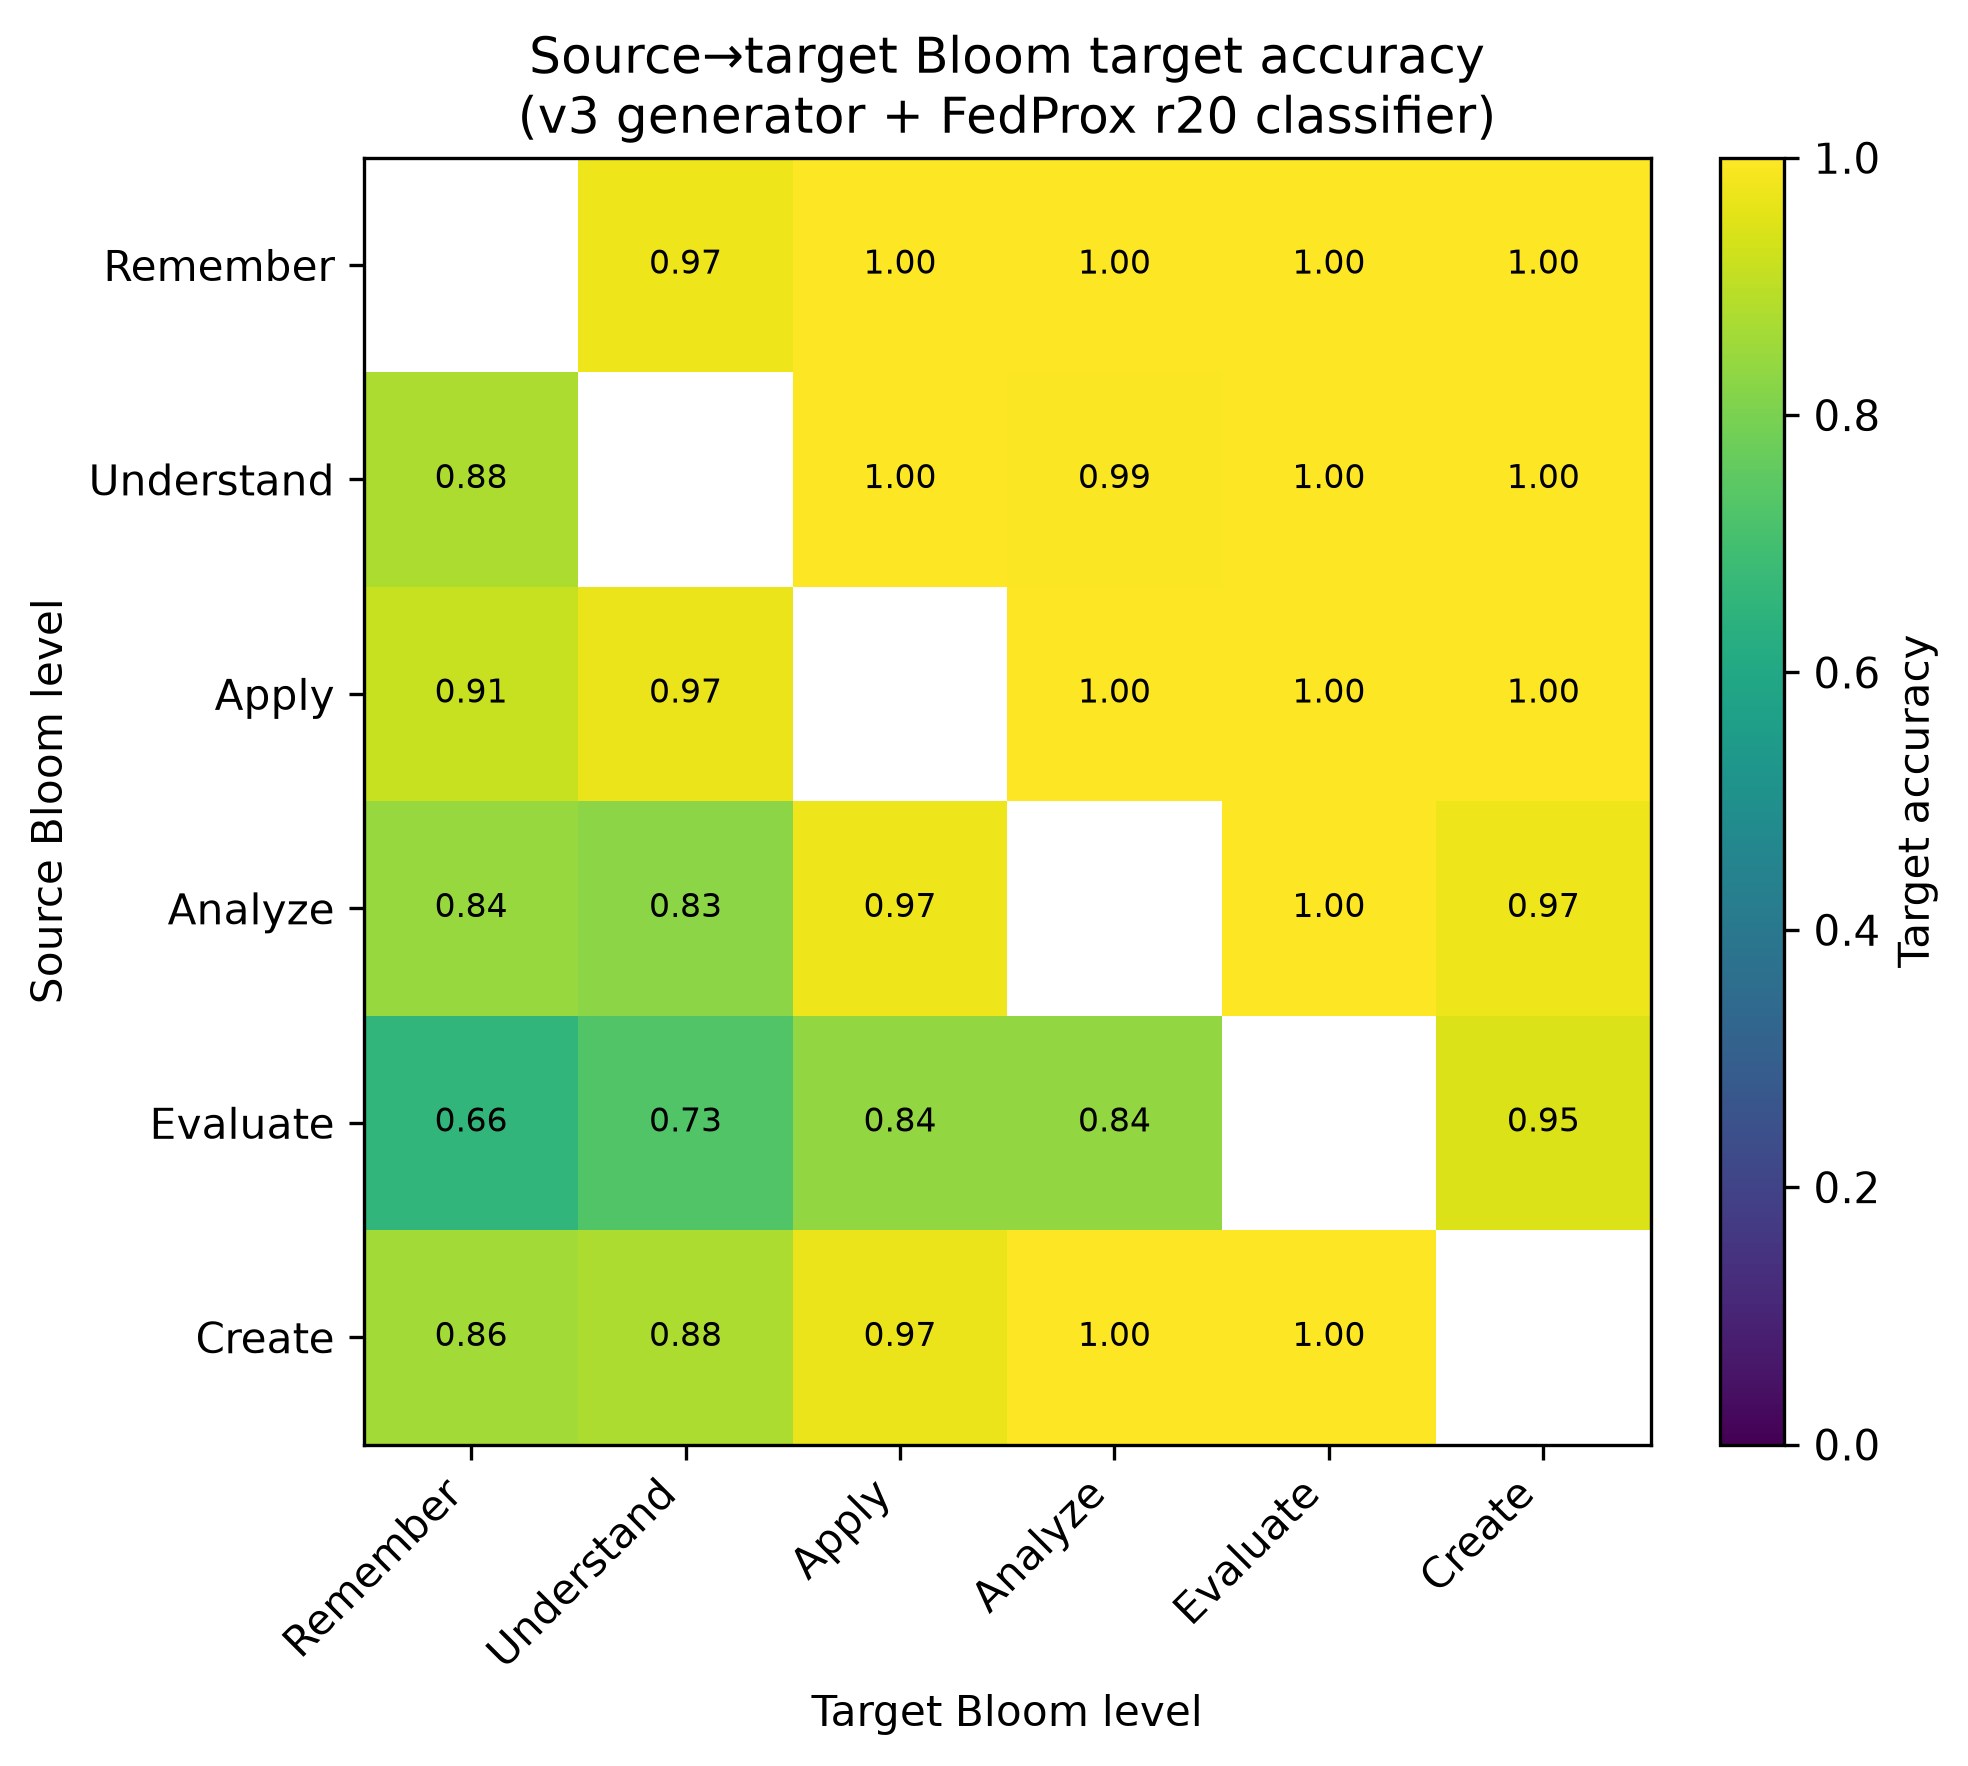
\includegraphics[width=\columnwidth]{fig04_source_target_accuracy.png}
\caption{Source$\rightarrow$target target-accuracy heatmap (v3 + FedProx scorer).}
\label{fig:st}
\end{figure}

\begin{figure}[t]
\centering
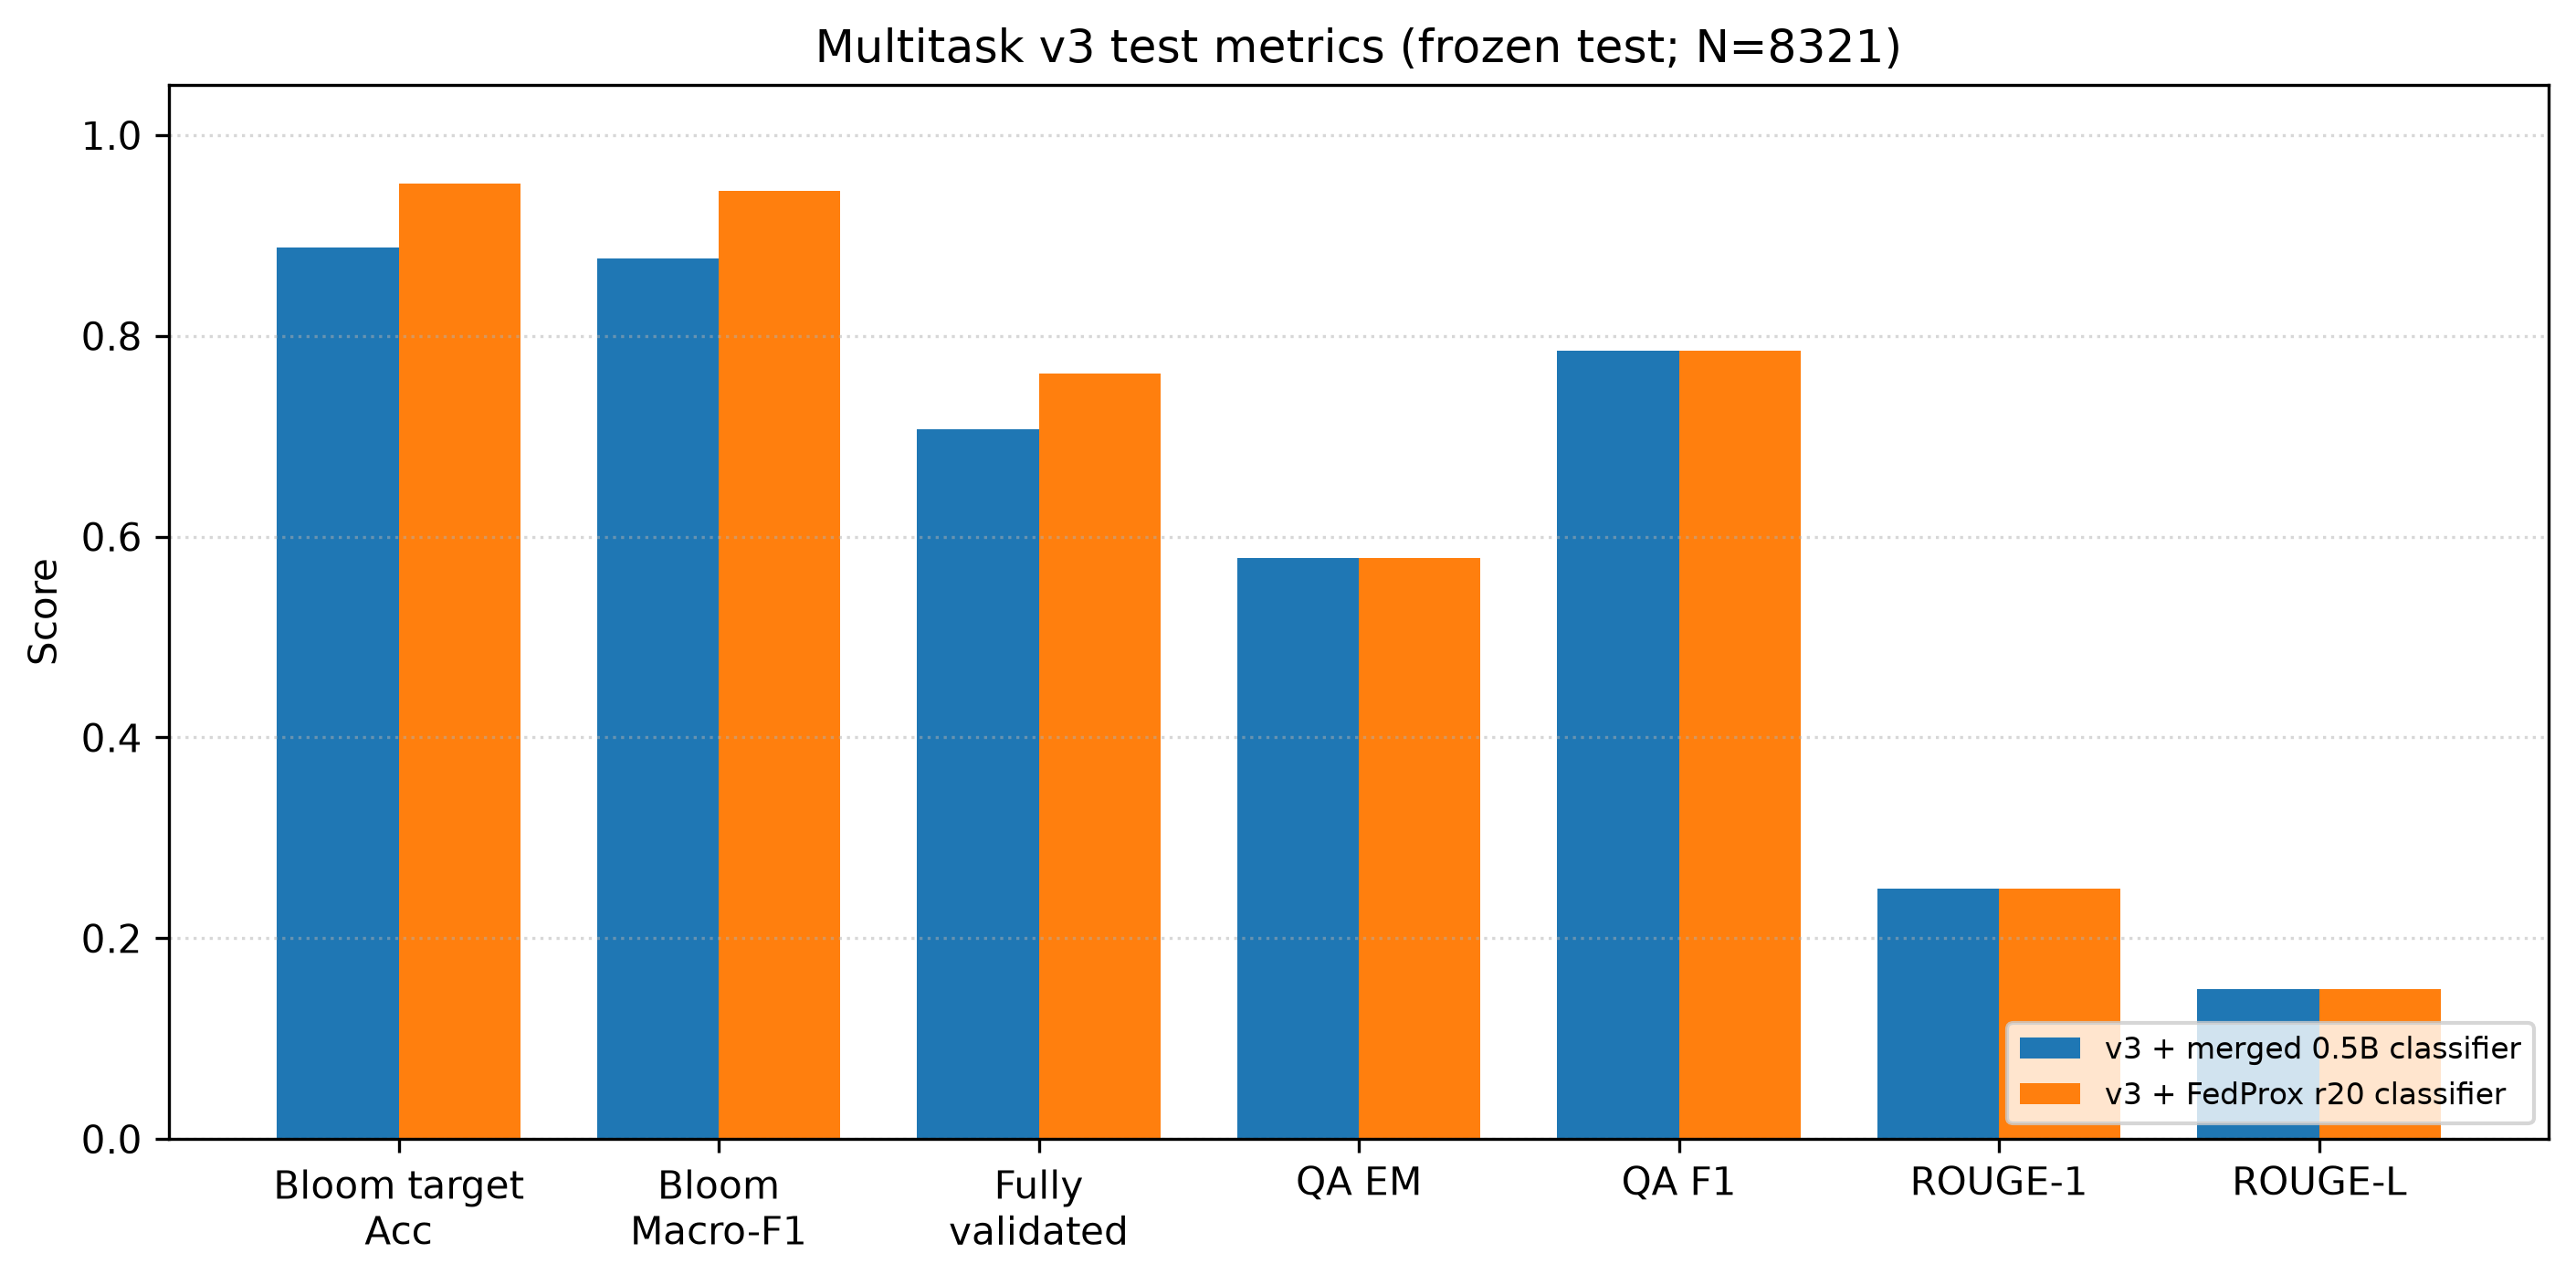
\includegraphics[width=\columnwidth]{fig06_multitask_task_performance.png}
\caption{Task-level comparison for v3 under two classifier scorers.}
\label{fig:mtbars}
\end{figure}

\subsection{Deployment and privacy}
GGUF Q4\_K\_M: $986{,}048{,}032$ bytes; startup $0.687$~s; mean latency $0.6865$~s; $28.8944$ tokens/s; RSS $1300.01$~MB; USS $694.46$~MB (Fig.~\ref{fig:gguf}).
PrivacyGuard: attack block rate $1.0$ ($104/104$); benign allow rate $0.0$ ($15$ prompts).
No complete quantitative EduGuard RAG benchmark exists in the repository; only smoke-scale rows should be acknowledged if mentioned at all.

\begin{figure}[t]
\centering
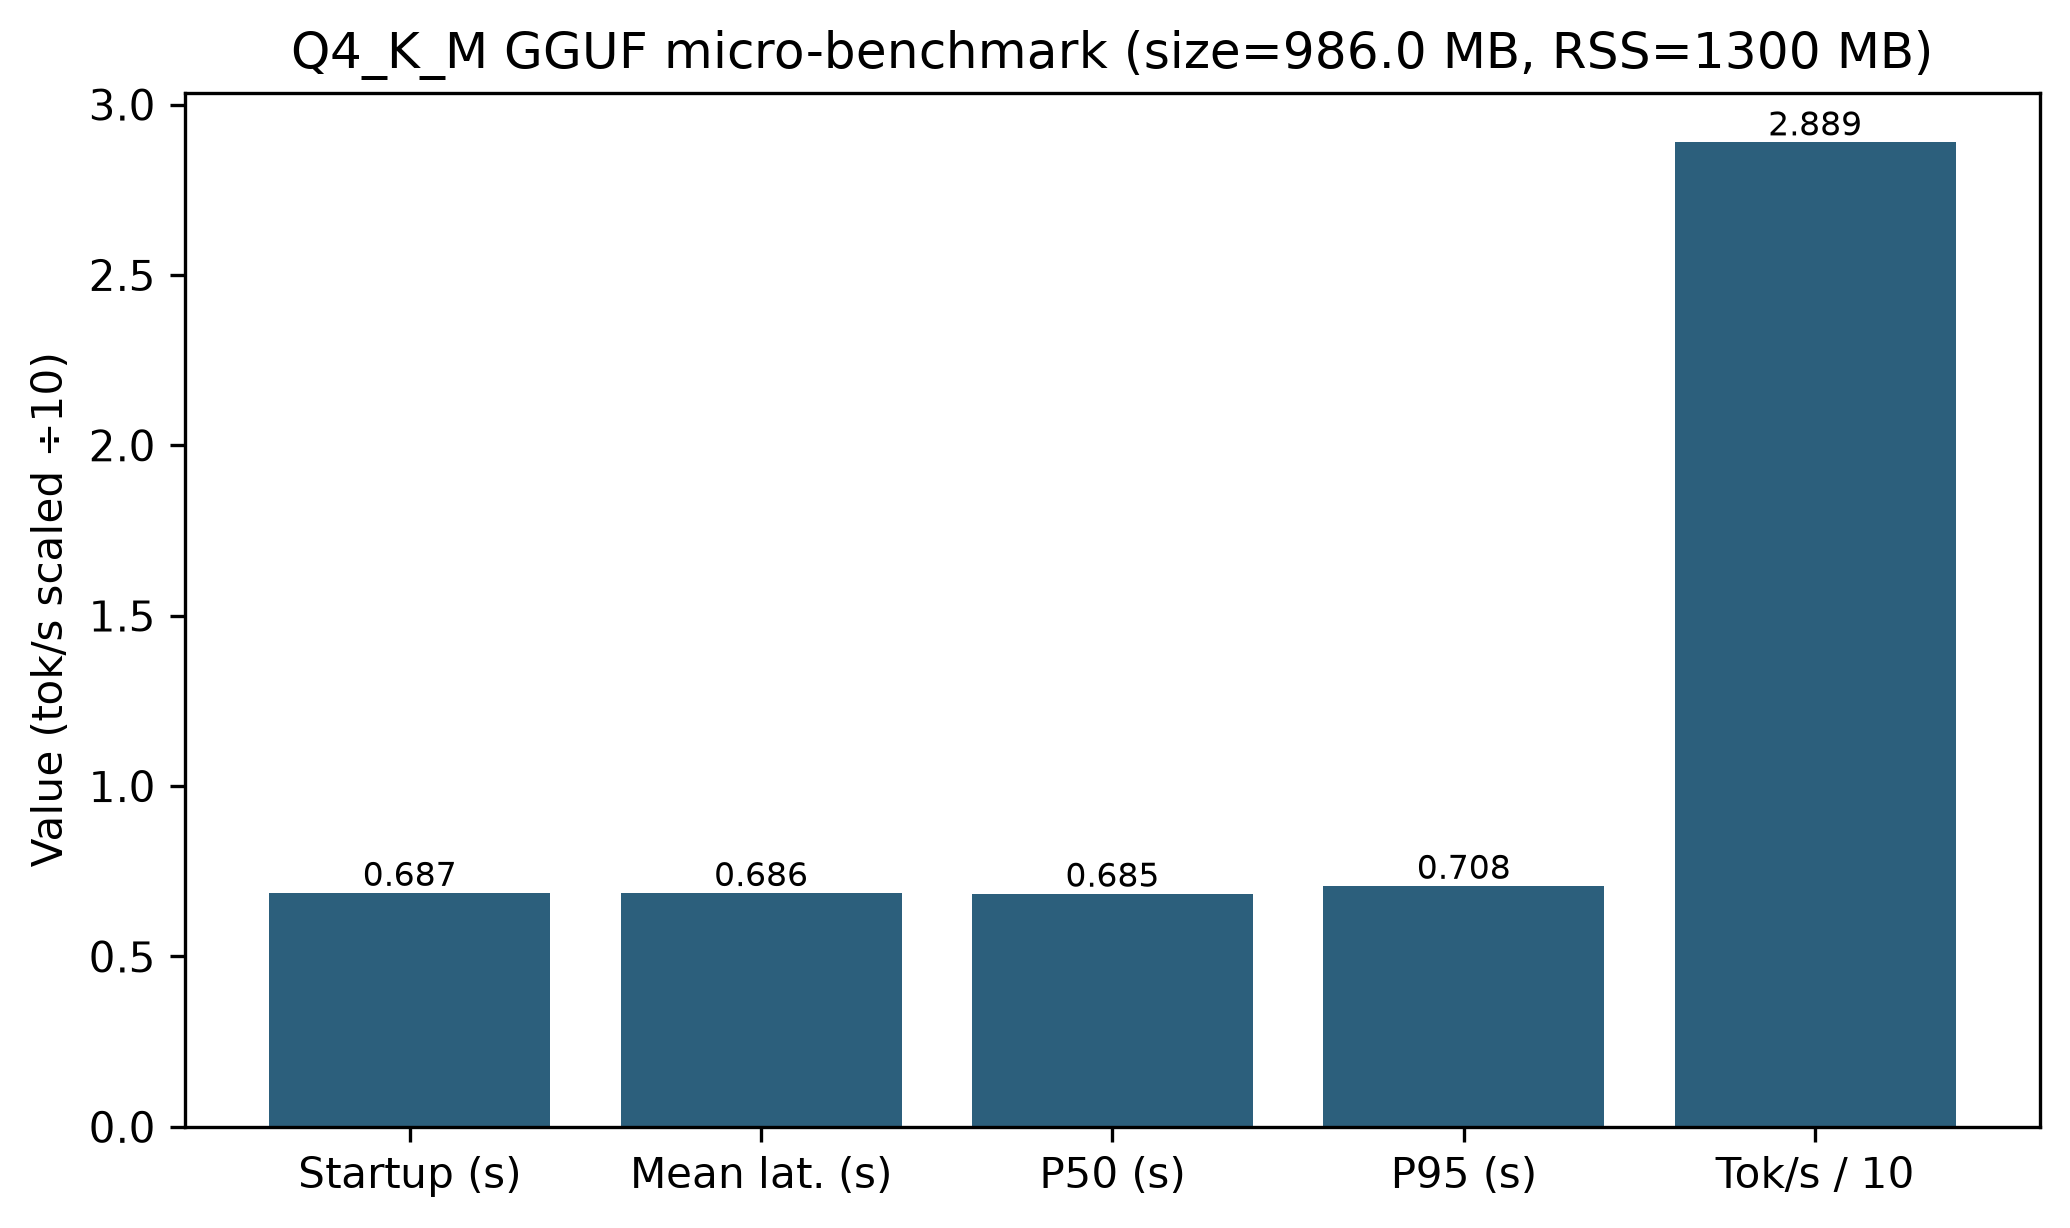
\includegraphics[width=\columnwidth]{fig07_gguf_deployment.png}
\caption{Q4\_K\_M micro-benchmark summary.}
\label{fig:gguf}
\end{figure}

\begin{figure}[t]
\centering
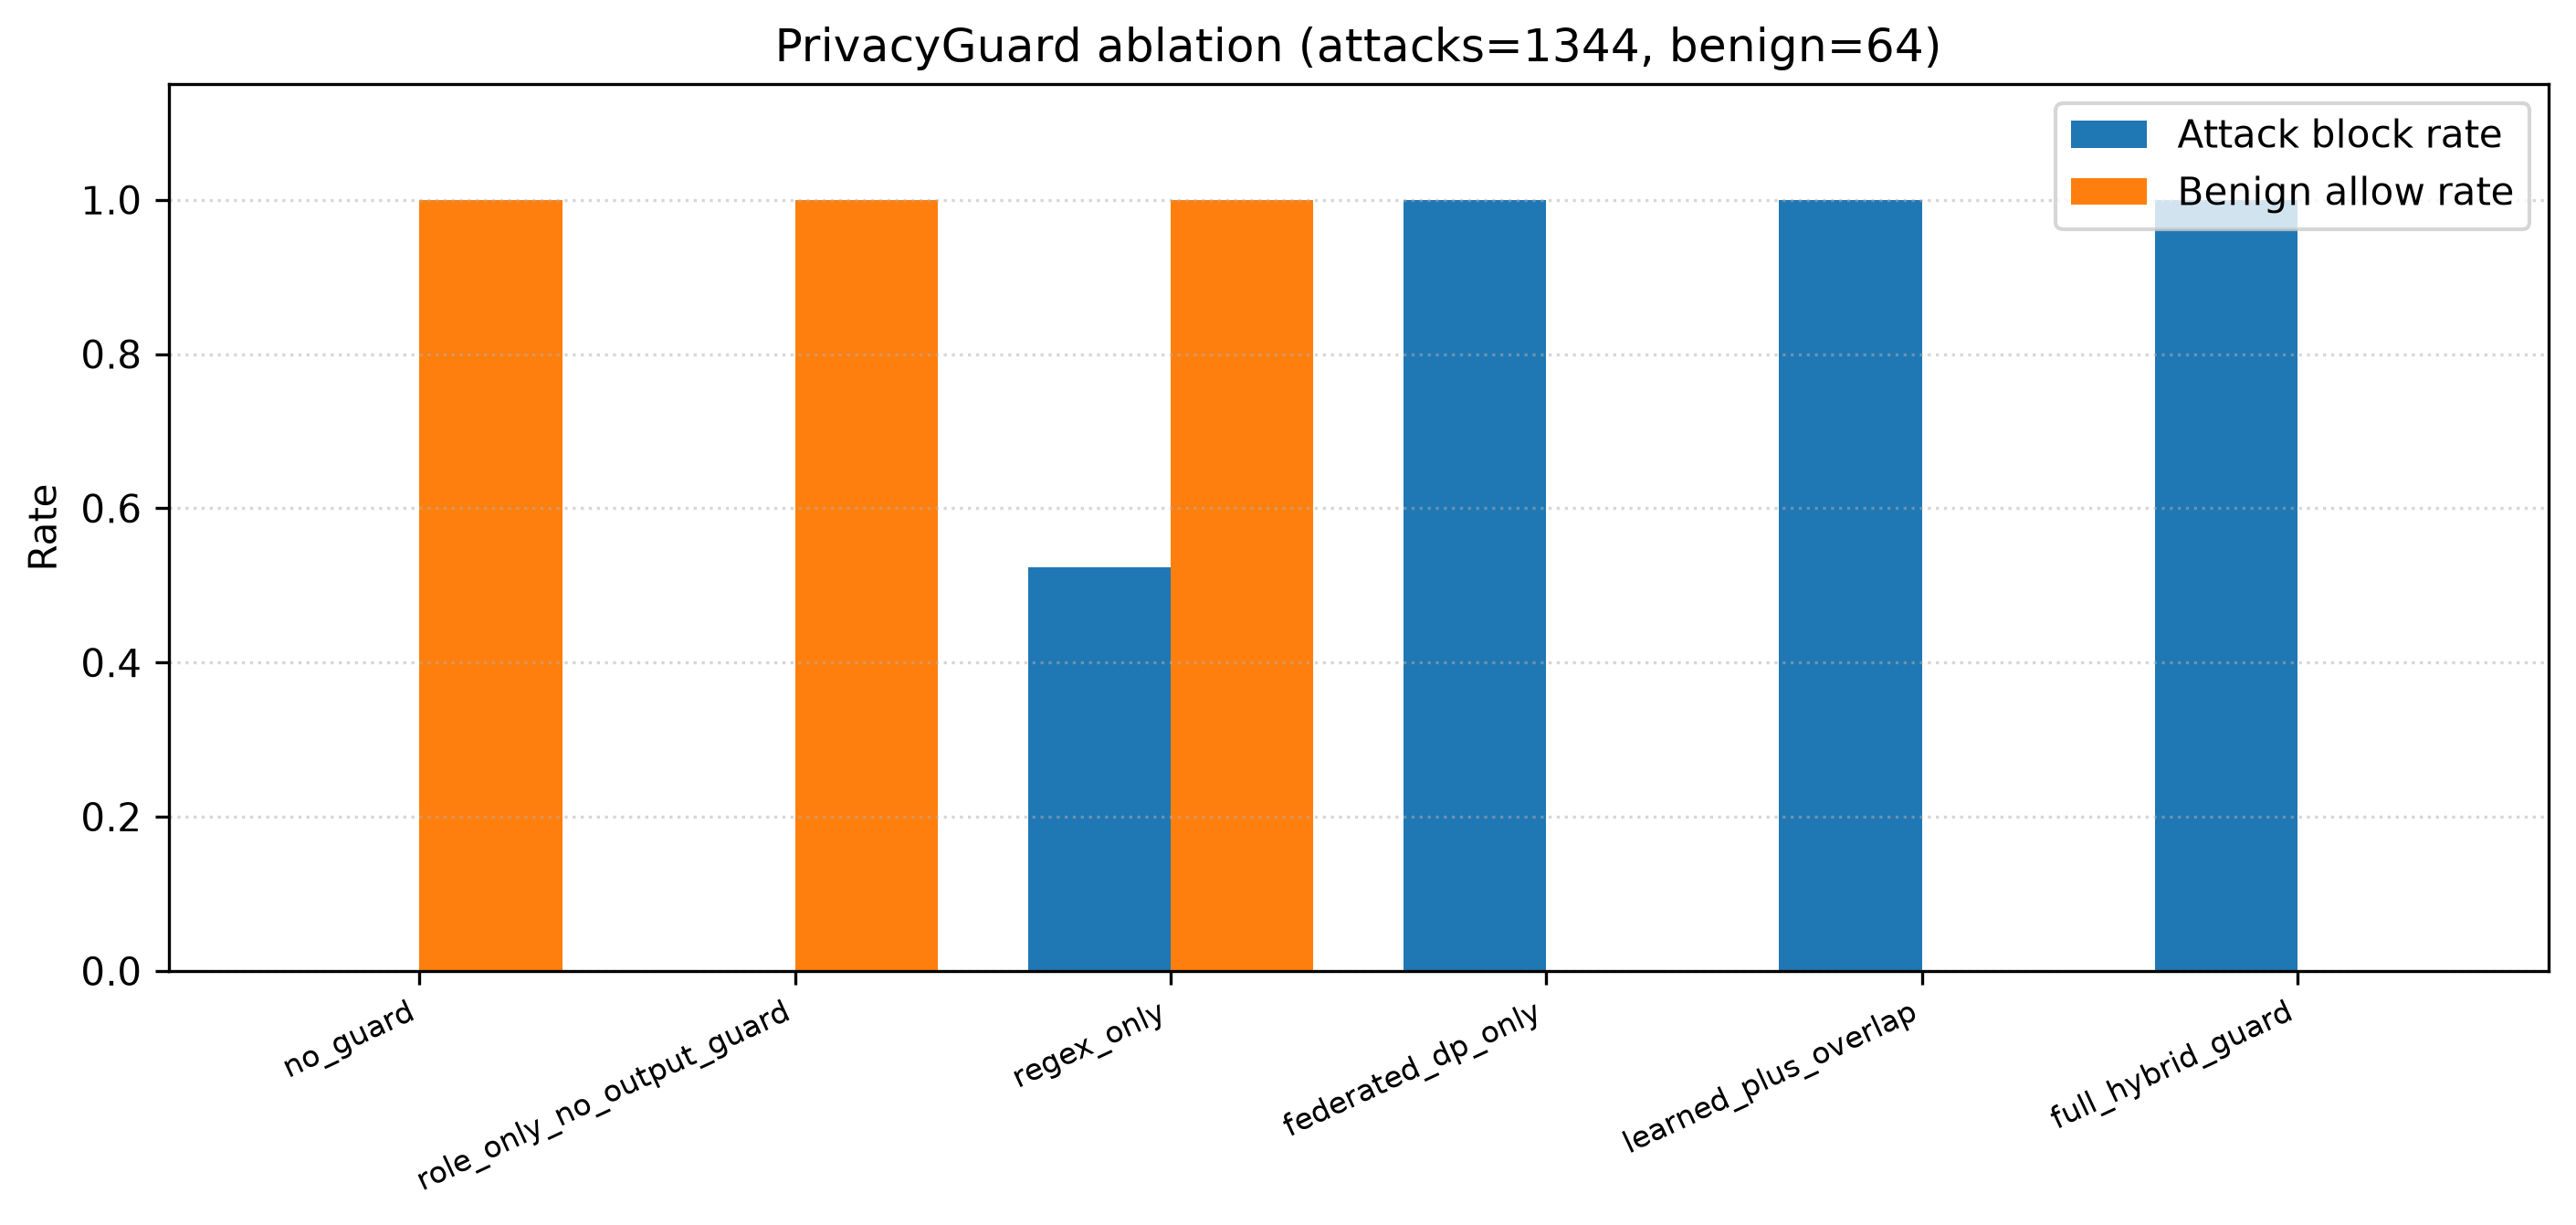
\includegraphics[width=\columnwidth]{fig08_privacy_ablation.png}
\caption{PrivacyGuard baseline ablation (attack block vs benign allow).}
\label{fig:priv}
\end{figure}

\section{Discussion}
The results support a pragmatic split: keep Bloom classification on a small federated sequence model, and keep generation on a separately trained 1.5B multitask checkpoint optimized for rewrite validation under v3.
Federated learning narrows---but does not eliminate---the gap to centralized accuracy under IID simulation.
On the tested non-IID split, FedProx does not outperform FedAvg at $\mu{=}0.01$, which should not be read as a general rejection of FedProx~\cite{li2020fedprox}.
The DP-SGD condition remains a negative utility result and is not part of the deployed system.
Privacy controls currently over-block benign traffic; that finding should guide threshold redesign rather than be omitted.

\section{Limitations}
Synthetic rewrite targets; missing human ratings; incomplete FedProx non-IID grid; DP-FL utility failure; absent full RAG/OCR benchmarks; possible missing weight binaries in partial checkouts; ECE dual values ($0.0537$ vs $0.0565$) requiring explicit disclosure.

\section{Conclusion}
EduGuard's publication evidence centres on FedProx-selected 0.5B Bloom classification, multitask v3 generation, Q4\_K\_M local deployment of the generator, and empirical PrivacyGuard behaviour with stated utility costs.
Reproducible tables and figures are regenerated by \texttt{scripts/final\_paper\_experiments.py} from locked artifacts without inventing metrics.

\section*{Supplementary material}
The attachable bundle is \texttt{paper/attachment/}, rebuilt by
\texttt{scripts/build\_paper\_attachment.py}.
It contains the eight figures, the final tables, the experiment inventory,
the validation report, and the proof-status files for retrieval and PrivacyGuard.
Model weights are not included.

\section*{Acknowledgements}
Add funding acknowledgements here.

\bibliographystyle{elsarticle-num}
\bibliography{references}

\end{document}
